\section{\textbf{E}ntity \textbf{R}elationship \textbf{D}iagram (ERD)}
\begin{spacing}{1}

    \begin{figure}[H]
        \centering
        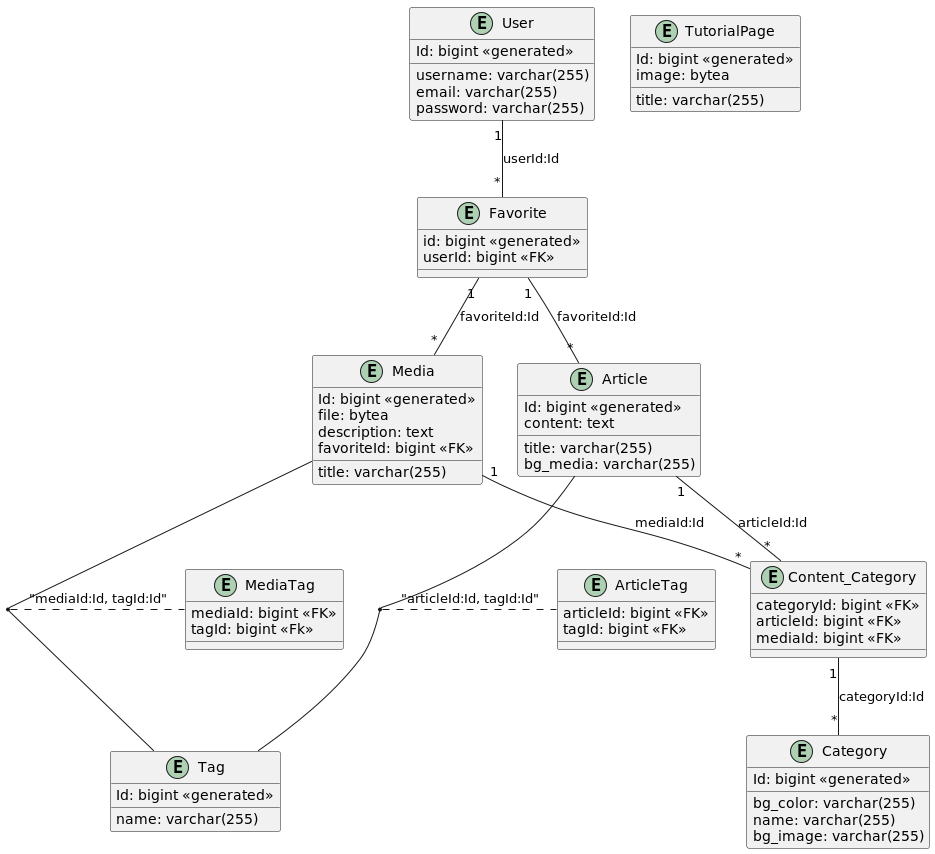
\includegraphics[height=1\textwidth]{./pics/erd.png}
        \caption{ERD}

    \end{figure}
\end{spacing}


\section{Medias und Articles}

Grundsätzlich haben wir als Team entschieden,
die Artikeln und die Medien in zwei speraten Tabellen zu speichern,
da Artikeln mehrere Bilder, Videos und Audios Inhalte enthalten können.
Diesen können dann mittels ein "Rich Text Editor" hinzugefügt werden.
Bei "Media" handlet es sich nur um ein Medienelement,
nähmlich ein Bild, Video oder Audio File. Es ist aber wichtig anzumerken,
dass keine Benutzeroberfläche für die Artikeln implementiert wurde, da der Kunde
diese nicht in dem \textbf{M}inimal \textbf{V}iable \textbf{P}roduct (MVP) haben wollte.
Für die Relaisierung des kompletten Datenmodels war aber das Einfügen der Artikel erforderlich.

\section{TutorialPage}
Die Entität "TutorialPage" hat keine Beziehungen zu anderen Entitäten, da sie nur für den Inhalt des Tutorial-Slideshows,
die nach der erfolgreichen Installation der App angezeigt wird, gedacht ist.

\begin{figure}[H]
    \centering
    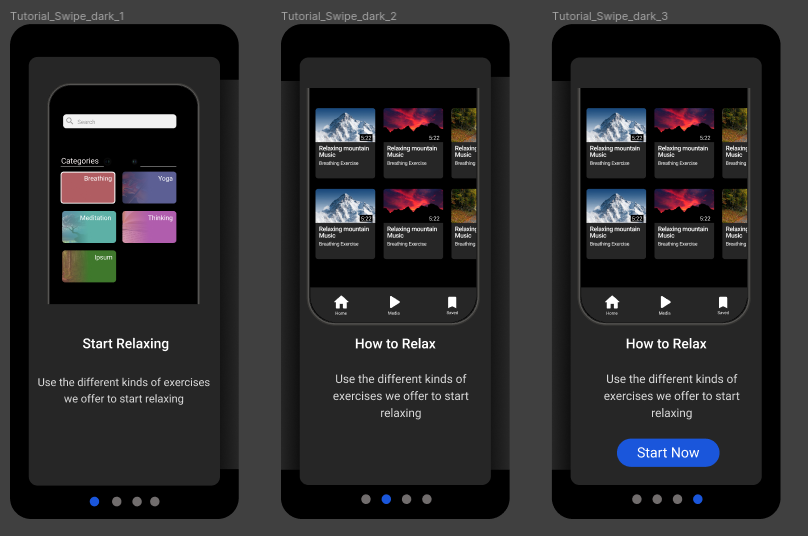
\includegraphics[height=0.5\textwidth]{./pics/slideshow.png}
    \caption{Screenshot aus dem UI Prototyp von Relaxoon}
\end{figure}

Mit der Persestierung der Inhalte von der Slideshow könnte die Erstellung
von neuen Builds bei jeder Änderung vermieden werden.


\section{Suche und Filterungen}

Bei den Filterungen wurde der "Interactive Query Builder" verwendet,
um die Filterparameter der Abfragen zu generieren
und diese dann bei den REST Abfragen anzuhängen.
Es gibt auch eine "Query Engine", welche die gleiche Funktion wie diese
"Interactive Query Builder" hat.
Diese kann in dem \textbf{O}bject \textbf{R}elational \textbf{M}apper (ORM) angewendet werden.
Mit der Verwendung dieser "Interactive Query Builder" kann man die Daten,
die man von den REST-Resourcen bekommt, anpassen.
Es gibt auch die Möglichkeit, die REST-Resource im Backend mittels dieser
"Query Engine" anzupassen.
Allerdings wurde diese "Query Engine" nicht verwendet,
da die Dokumentation bzw. Intellisense von dem ORM sehr ungenau war.

\begin{figure}[H]
    \centering
    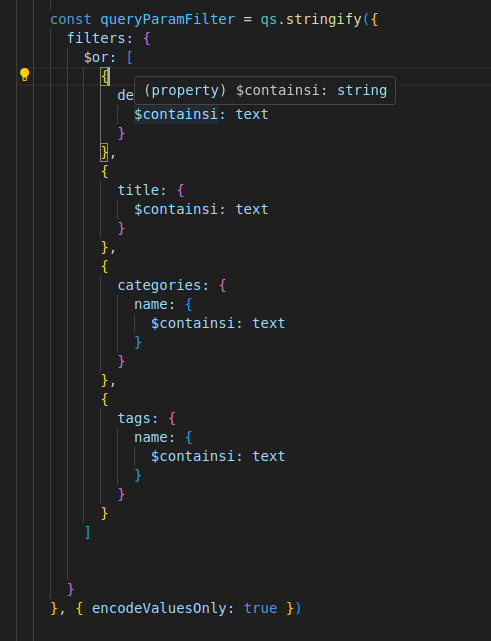
\includegraphics[ width=1\textwidth]{./pics/query-builder.png}
    \caption{Beispiel für den Interactive Query Builder}
\end{figure}




\begin{spacing}{1}
    \textbf{API-Route mit den angehängten generierten Abfrageparameter}:
    \newline
    \textcolor{red}{/medias?\&populate[tags]=true
    \&populate[file]=true
    \&populate[favorite][populate]=\newline users\_permissions\_user}
\end{spacing}







% Siehe tolle Daten in Tab. \ref{tab:impl:data}.

% \begin{table}
%     \centering
%     \begin{tabular}{|lcc|}
%     \hline
%               & \textbf{Regular Customers} & \textbf{Random Customers} \\ \hline
%     Age       & 20-40                      & \textgreater{}60          \\ \hline
%     Education & university                 & high school               \\ \hline
%     \end{tabular}
%     \caption{Ein paar tabellarische Daten}
%     \label{tab:impl:data}
% \end{table}

% \begin{figure}
%     \centering
%     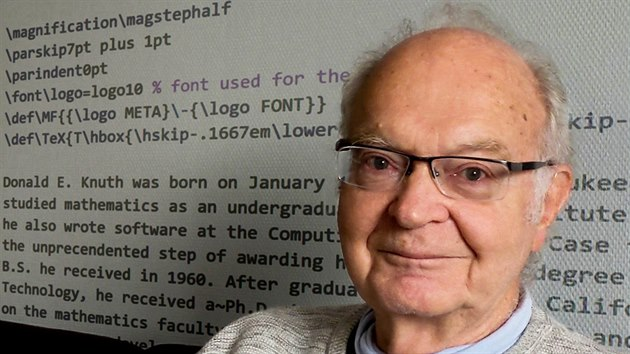
\includegraphics[scale=0.5]{pics/knuthi.jpg}
%     \caption{Don Knuth -- CS Allfather}
%     \label{fig:impl:knuth}
% \end{figure}

% Siehe und staune in Abb. \ref{fig:impl:knuth}.
% \lipsum[6-9]
% Dann betrachte den Code in Listing \ref{lst:impl:foo}.

% \begin{lstlisting}[language=Python,caption=Some code,label=lst:impl:foo]
% # Program to find the sum of all numbers stored in a list (the not-Pythonic-way)

% # List of numbers
% numbers = [6, 5, 3, 8, 4, 2, 5, 4, 11, 33]

% # variable to store the sum
% sum = 0

% # iterate over the list
% for val in numbers:
%     sum = sum+val

% print("The sum is", sum)
% \end{lstlisting}